\chapter{\texorpdfstring{$\cN=2$ Dualities}{Gaiotto theories}}
We study $\cN=2$ gauge theories which have exactly marginal deformations. The starting point is typically a UV lagrangian and the purpose of the game is to understand the properties of the theory by exploring the moduli space of vacua. We want to see what happens if also the UV theory has a moduli-space of parameters which we can play with.\\
Of course for each point we have a theory and we can ask what is the IR dynamics by exploring the moduli-space of vacua. So to each point of the UV moduli-space of parameters we have some moduli space for the IR description fibered over it.

For the $\SU(2)$ theory we had that the moduli-space of vacua was parametrized by a complex parameter $u$ and for $u\gg\Lambda$ the theory is weakly coupled and using holomorphicity we can start studying the interior and get the full description on the whole moduli space. One has to pay a prize to go into the moduli space: in the weakly coupled limit we have some lagrangian but going in one encounters singularities and monodromies and one has to go to an equivalent description where the gauge coupling is again weak.\\
One ends up with a sort of manifold of lagrangian description, with various patches with simple lagrangian description and moving between them we have to use some EM dualities. We cannot describe everything with only one lagrangian.

This is what we expect to happen also in the UV. So we start in some corner of the moduli-space where all the couplings are weak in some lagrangian description, then we start dyiliyg the couplings to make them strong and move to some strong coupling region and we find ourselves in another weakly coupled region with some other lagrangian description and so on. We find many weakly coupled descriptions in various corners of the moduli-space by tuning the couplings. At the end one tries to fill in to find a whole description in terms of weakly coupled lagrangian descriptions.

To understand this structure, we need to understand very well the weakly coupled regions. So what is the most general renormalizable $\cN=2$ lagrangian?  This amount of susy is enough to answer this question. We have vector multiplets (in $\cN=1$ this is a vector multiplet plus a chiral adjoint multiplet) and hypermultiplets (this is a combination of two chiral multiplets in conjugate rep of the gauge group). It turns out that the $\cN=2$ susy, the interactions are only the supersymmetric partners of gauge interactions. Once I have the gauge group $\prod_{i}G_{i}$ and what are the matter representations $\bigoplus_{I}n_{I}(R_{I}\oplus \bar R_{I})$ the general structure of the lagrangian is determined. The only freedom is putting gauge couplings and masses. There is a particularly important interaction (in $\cN=1$ language) which is the superpotential 
\begin{equation}
	\cW=Q_{s}^{i}\phi_{i}^{j}\tilde Q_{{j}}^{s}+M_{t}^{s}Q_{s}^{i}\tilde Q_{i}^{t}
\end{equation}
where we have some hypermultiplets $Q,\tilde Q$, some adjoint scalars $\phi$ and a mass term $M$ (in some adjoint of the flavour symmetry). Flavour symmetries will play a very important role. The superpotential is invariant by $s,t$ index rotations so we always have some $\prod_{I}\U(n_{I})$ flavour symmetry at least if $R_{I}$ is some complex representation. But if the rep is real or pseudoreal, one can try to rotate together $Q,\tilde Q$ but due to the coupling one cannot rotate them freely. If $R_{I}$ is real, then the adj rep can be represented by anti-symmetric matrices, putting $\hat{Q}=(Q,\tilde Q)$
\begin{equation}
	\cW\supset \phi_{\comm{i}{j}}\hat{Q}^{i}_{s}\hat{Q}^{j}_{t}\omega^{st}
\end{equation}
where $\omega^{st}$ is some symplectic form to make the term non-vanishing. So whatever flavour symmetry we have, it must preserve this symplectic form. So if the rep is real, the flavour symmetry is enhanced to $\USp(2n_{I})$. Instead, if $R_{I}$ is pseudoreal, then the adjoint fields can be written in the way that the have symmetric indices 
\begin{equation}
	\cW\supset \phi_{(i,j)}\hat{Q}^{i}_{s}\hat{Q}^{j}_{t}\eta^{st}
\end{equation}
where $\eta^{st}$ is a symmetric form that has to be preserved. Therefore the flavour group is enhanced to $\SO(2n_{I})$. It's worth mentioning that if the rep is pseudoreal, one can try to keep half of the matter content so that one has an $\SO(2n_{I}+1)$. Classically always works, but quantum mechanically it is not given (anomaly: the determinant of the hyperinos can have a sign ambiguity under large gauge transformations).

Every time one has a flavour symmetry, we can add a mass parameter. But initially when we descrive the UV theory, we want the conformal case so we turn it off. Then we can turn it on an descrive the IR physics of the theory. How do I know if a gauge coupling is exactly marginal? In $\cN=2$ theories we know that the gauge coupling is renormalized at 1-loop but we assume that there are no non-perturbative corrections. If there is no matter, the theory is asymptotically free automatically. By adding matter the beta function becomes smaller and the theory becomes less and less asymptotically free. At some point it becomes IR free and a Landau pole appears. By putting just the right amount of matter, the beta function vanishes and there are no corrections so the coupling is marginal. What is this right amount of matter? For any gauge group $G$ we can take the rep to be the adjoint and then the beta function vanishes (this gives $\cN=4$ supersymmetric theory).\\
Another possibility is with $\SU(N)$ gauge groups and add $2N$ fundamental flavours $R=\sum 2N R_{fund}$. This will give a flavour symmetry $\SU(2N)$.\\
There is a variation where $G=\SU(N_{1})\times \SU(N_{2})$: we can add a bifundamental which counts as $N_{1}$ copies of a fundamental for $\SU(N_{2})$ and $N_{2}$ copies of a fundamental for $\SU(N_{1})$. So with several unitary gauge groups, one can take several combinations of bifundamentals to make the beta function vanish. For example

\begin{equation}
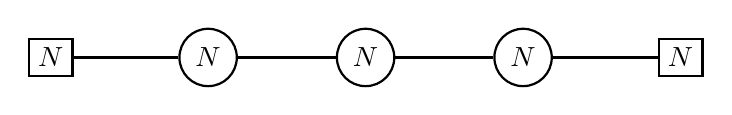
\begin{tikzpicture}[thick]
  \node[circle,draw] (one) at (0,0) {$N$};
  \node[circle,draw]  (two) at (2,0) {$N$};
  \node[circle,draw]  (three) at (4,0) {$N$};
  \node[rectangle,draw]  (flav1) at (-2,0) {$N$};
  \node[rectangle,draw]  (flav2) at (6,0) {$N$};
  \draw[-](one)--(two);
  \draw[-](two)--(three);
  \draw[-](one)--(flav1);
  \draw[-](flav2)--(three);
\end{tikzpicture}
\end{equation}
All the gauge couplings are exactly marginal since each gauge group has $2N$ flavours. The flavour symmetry of this theory is $\U(1)\times\U(1)\times\U(N)\times\U(N)$, where the $\U(1)$s come from the bifundamentals and the $\U(N)$s come from the fundamentals at the start and and of the quiver.\\
One can generate many more examples like this, for example
\begin{equation}
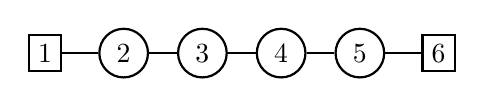
\begin{tikzpicture}[thick]
  \node[circle,draw] (one) at (0,0) {$2$};
  \node[circle,draw]  (two) at (1,0) {$3$};
  \node[circle,draw]  (three) at (2,0) {$4$};
  \node[circle,draw]  (four) at (3,0) {$5$};
  \node[rectangle,draw]  (flav1) at (-1,0) {$1$};
  \node[rectangle,draw]  (flav2) at (4,0) {$6$};
  \draw[-](one)--(two);
  \draw[-](two)--(three);
  \draw[-](three)--(four);
  \draw[-](one)--(flav1);
  \draw[-](flav2)--(four);
\end{tikzpicture}
\end{equation}
where, again, all the gauge couplings are marginal. One could ask why we do not branch around, but mathematically the shape of the graph is quite constrained by the requirement on the number of flavours. This is very similar to what happens with Dinkin diagrams in Lie algebras. The conformal quivers will always look like a sequence of gauge groups or that it bifurcates at the ends, or a loop (affine Dinkin diagrams). One can also get some exeptional diagrams.

One could also start to play with the gauge groups by looking at real groups: for $\USp(2N)$ we need $2N+2$ fundamentals so that the flavour group is $\SO(4N+4)$. The same can be said with an $\SO(2N)$ with $2N-2$ flavours. These allow to make quivers alternating $\USp$ and $\SO$ groups with half hypers connecting them. The continuous flavour symmetry will be just the one at the end of the quivers.

With a little bit of combinatorial work one can write down all the superconformal $\cN=2$ lagrangians with marginal couplings. What are the most general $\cN=2$ SCFT with gauge group $G=\SU(2)^{n}$? Let us write down some examples: 
\begin{enumerate}
	\item $\SU(2)$ with one adjoint is $\cN=4$ susy gauge theory. 
	\item $\SU(2)$ with $4$ fundamentals $N_{f}=4$, has $\SO(8)$ flavour symmetry.
\end{enumerate}
this is all with one gauge group. Let us go to two, beside trivial possibility of taking decoupled product of the last ones, 
\begin{equation}
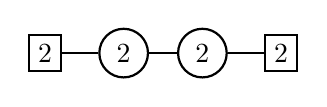
\begin{tikzpicture}[thick]
  \node[circle,draw] (one) at (0,0) {$2$};
  \node[circle,draw]  (two) at (1,0) {$2$};
  \node[rectangle,draw]  (flav1) at (-1,0) {$2$};
  \node[rectangle,draw]  (flav2) at (2,0) {$2$};
  \draw[-](one)--(two);
  \draw[-](one)--(flav1);
  \draw[-](flav2)--(two);
\end{tikzpicture}\qquad
\begin{tikzpicture}[thick,decoration={
    markings,
    mark=at position 0.6 with {\arrow{>>}}}]
  \node[circle,draw] (one) at (0,0) {$2$};
  \node[circle,draw]  (two) at (2,0) {$2$};
  \draw[postaction={decorate}](one)--(two);
\end{tikzpicture}
\end{equation}
For the right one, one would think to have a $\U(2)$ flavour symmetry, but since the fundamental rep is pseudoreal, then the product of two fundamentals is real so we actually have a $\USp(4)$ flavour symmetry. The left one is more typical: there is a $\SO(4)^{2}$ coming from external fundamentals, while from the bifundamental there is a $\USp(2)$. But really the flavour group is $\SU(4)^{5}$ since $\SO(4)\sim\SU(2)\times\SU(2)$ and $\USp(2)\sim\SU(2)$.\\
Notice also that a pair of bifundamentals $(Q,\tilde Q)$ can be combined into one single $\hat Q$ which carries a $\USp(2)$ index
\begin{equation}
	\hat Q_{i_{1}i_{2}a}
\end{equation}
just writing $8=2\times2\times2$. These three indices play the same roles but the first two are gauged. But there is no reason to why I shouldn't be able to gauge other ones. We represent this object as a junction
\begin{equation}
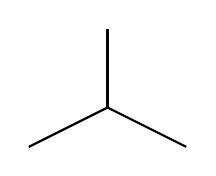
\begin{tikzpicture}[thick]
  \draw[-](0,0.5)--(0,-0.5);
  \draw[-](0,-0.5)--(-1,-1);
  \draw[-](0,-0.5)--(1,-1);
\end{tikzpicture}
\end{equation}
This adds two fundamental to every gauge group, but marginallity requires four fundamentals, and so we need two blocks, for example the $\SU(2)$ $N_{f}=4$ case is given by
\begin{equation}
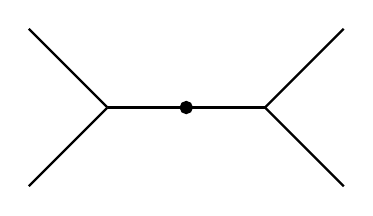
\begin{tikzpicture}[thick]
  \draw[-](0,0)--(1,-1);
  \draw[-](1,-1)--(0,-2);
  \draw[-](1,-1)--(2,-1);
  \draw[-](2,-1)--(3,-1);
  \draw[-](3,-1)--(4,0);
  \draw[-](3,-1)--(4,-2);
  \filldraw[black] (2,-1) circle (2pt) node[]{};
\end{tikzpicture}
\end{equation}
where the dot means the gauged group. We can also see, at least a subgroup, of the flabvour symmetry: in fact it is manifest an $\SU(2)^{4}\sim \SO(2)^{2}\subset \SO(8)$ flavour symmetry.

With this basic building block I can construct much more complicated theories. For any threevalent graph $\Gamma$ one gets a theory $T_{\Gamma}$ labelled by the graph. There are a couple of exeptional situations: take for example the following
\begin{equation}
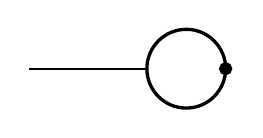
\begin{tikzpicture}[thick]
	\draw[-](0,0)--(1.5,0);
	\filldraw[color=black, fill=white, very thick](2,0) circle (0.5);
 	\filldraw[black] (2.5,0) circle (2pt) node[]{};
\end{tikzpicture}
\label{eq:N4}
\end{equation}
where two of the flavour symmetries are identified and gauged. What happens when we decompose $2\times 2\times 2a$? The first two give an adjoint plus a singlet that is not gauged. So this picture is $\SU(2)$ $\cN=$ plus a floating singlet. The singlet is important since now we can do 
\begin{equation}
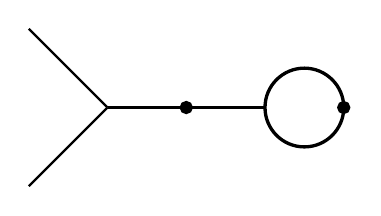
\begin{tikzpicture}[thick]
  \draw[-](0,0)--(1,-1);
  \draw[-](1,-1)--(0,-2);
  \draw[-](1,-1)--(2,-1);
  \draw[-](2,-1)--(3,-1);
  \filldraw[color=black, fill=white, very thick](3.5,-1) circle (0.5);
  \filldraw[black] (4,-1) circle (2pt) node[]{};
  \filldraw[black] (2,-1) circle (2pt) node[]{};
\end{tikzpicture}
\end{equation}
the adjoint, from the point of view of the central gauge group, looks like $3/2$ of a fundamental but with the singlet we have another $1/2$ fundamental that we can therefore gauge.

Let us discuss some of the properties of these theories $T_{\Gamma}$. Suppose to have $n$ external legs and $g$ loops. Without loops is very easy to count vertices and internal legs. Every loop removes two external legs and adds a vertex. Therefore we have $\SU(2)^{3g-3+n}$ gauge group. In particular there are going to be $3g-3+n$ gauge couplings $\tau_{i}$. There are also going to be $3g-3+n$ order parameters for the IR theory $\Tr\phi_{i}^{2}$ (coulomb branch order parameters).Notice that these order parameters and gauge couplings are intimately connected: if I want to change the gauge coupling I just take the lagrangian and add a prepotential term
\begin{equation}
	L+\delta\tau_{i}\int\dd[2]{\theta}\dd[4]{x}\Tr\phi^{2}_{i}
\end{equation}
There is also a flavour symmetry group $\SU(2)^{n}$, one for every external leg. In particular there are the mass parameters for this flavour group $\Tr M^{a}_{b}$. The mass parameter and the Coulomb branch scalars enter in the same way, so the mass parameters are just the order parameters for very weakly gauged flavour group.\\
For every $n,g$ the skeleton of the theory is the same, but they differ in how the matter couple.

\section{S-dualities}
We need to understand the S-dualities for these theories. We start from the simple cases. Consider $\cN=4$ $\SU(2)$ gauge theory. By moving in the Coulomb branch, the central charge $Z$ is uncorrected. The particles that move around in the Coulomb branch are: a W-boson (vector multiplet + hypermultiplet) which is half-BPS which has electric charge $1$ and magnetic charge $0$. At weak coupling it has a relatively small mass $Z=a$. Moving in the coulomb branch, we produce more particles. For example there is a magnetic monopole, half-BPS, and sit in the same multiplet as the $W$-boson but they have magnetic charge $1$ and electric charge $0$. It has a very heavy mass in the weak coupling limit $Z\sim \tau a$, but as $\tau\rightarrow 0$ they become lighter and lighter, becoming lighter than the $W$-boson. So in this limit, it does not make sense to think about the $W$-boson as the fundamental particle and as the monopole as some derived one. So we conjecture the existence of some sort of EM duality which exchanges them. The first test that this might be true, came out from looking at the full spectrum of magnetic monopoles and dyons. By quantizing one finds dyons $q_{M}=1$ and $q_{e}=n$. There are also magnetic monopoles with $q_{M}=2$ and dyons with $q_{e}=2n+1$. By going further one finds that there is a whole lattice of particles with electric and magnetic charges which are coprime $\gcd(q_{e},q_{m})=1$. By requiring that there is no wall crossing for half-BPS states, which means that the weakly coupled spectrum is actually the spectrum everywhere, we see that we have a spectrum of particles which is invariant under $\tau\rightarrow M\tau$ with $M\in \SL(2,\bbZ)$. This gives us a lot of weakly coupled regions which are divided by some strongly coupled regions.

One might wonder if the gauge coupling of the IR from which one can find the mass of the light fields, is the same parameter of the UV lagrangian. But this is an ill-defined question since the answer depends on the renormalization scheme. But we choose a renormalization scheme, when the masses are turned off, to have $\tau^{UV}=\tau^{IR}$.

Without wall crossing, we expect that the IR S-duality is still a symmetry in the UV since the spectrum of half-BPS states is the same.

Let us consider now the following theory $\SU(2)$ with $N_{f}=4$ flavours, which has $\SO(8)$ flavour symmetry. If the mass parameters, which sit in the cartan of $\SO(8)$, are turned off and if the vev of $\phi$ is zero, this theory has an exactly marginal gauge coupling $\tau$. By giving $\langle\Tr\phi^{2}\rangle=2a^{2}$ then, the central charge function cannot be corrected
\begin{equation}
	Z=(q_{e}+\tau^{IR}q_{m})a
\end{equation}
This theory seems to enjoy S-duality. But does the spectrum allow it? We have a $W$-boson ($q_{e}=2,q_{m}=0)$ plus a fundamental hypermultiplet which remember
\begin{equation}
	Q_{i}^{s}\tilde Q_{s}^{j}\phi^{i}_{j}
\end{equation}
becomes massless of mass $a$ and electric charge $1$. We have a flavour symmetry group which is unbroken so we label this particles by their $\SO(8)$ rep $\mathbf{8}_{v}$.\\
Surely there will be a classical solution in the Coulomb branch which is a smooth magnetic monopole solution with $q_{m}=1$ (quantizing it without flavour it is an hypermultiplet). With flavours there are more zero-modes: precisely there are $2N_{f}=8$ fermionic zero modes $\psi^{s}$ which transform in a vector of $\SO(8)$. What happens when we quantize them? We impose commutation relations
\begin{equation}
	\acomm{\psi^{s}}{\psi^{p}}=\delta^{sp}
\end{equation}
which tells us that these spinors are just gamma matrices that act on the monopoles: the monopole states live in spinor reps of the flavour group. Since the $\psi^{s}$ are also charged under the gauge group, they change the electric charge of the monopoles. The dyons
which have even electric charge sit in a positive chirality spinor and the ones with odd electric charge sit in a negative chirality spinor. There are also going to be particles with higher magnetic charges. Let us look just at the other ones for now.		
As $\tau\rightarrow\infty$ we are in the original weakly coupled limit, so we have a $W$-boson and hypermultiplet in $\mathbf{8}_{v,q_{e}}$. Then at $\tau=0$ we have monopoles in the spinor rep $\mathbf{8}_{s}$ while for $\tau=1$ we have ones in $\mathbf{8}_{c}$. This seems to be a problem but actually $\SO(8)$ has a $S_{3}$ outer automorphism group which exchanges these three representations\footnote{Symmetries of the Dynkin Diagram give rise to outer automorphisms of the Lie algebra. In the case where the Lie group is simply connected, such automorphisms are in one-to-one correspondance with group automorphisms. But when the Lie group is not simply connected all bets are off. Since $\pi_{1}(\SO(n))$ is of of order 2 (for $n>2$), some care must be taken. The second point is that the Dynkin Diagram of $\SO(8)$ actually has more symmetry, leading to the so called triality automorphism. This automorphism, in particular, maps $\text{Spin}(8)$, the universal covering, to itself and does not descend to $\SO(8)$.}. This is a good input by S-duality accompanied by the triality. In the fundamental region of the UHP we have three regions which are exchanged by the triality.

\subsection{Do the graph theory have S-dualities}
Let us start with the simplest theory $\SU(2)\times\SU(2)$

\begin{equation}
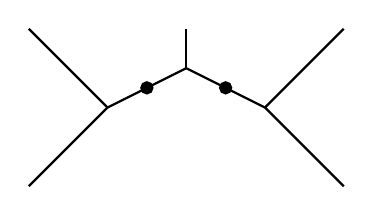
\begin{tikzpicture}[thick]
  \draw[-](0,0)--(1,-1);
  \draw[-](1,-1)--(0,-2);
  \draw[-](1,-1)--(2,-0.5);
  \draw[-](2,-0.5)--(2,0);
  \draw[-](2,-0.5)--(3,-1);
  \draw[-](3,-1)--(4,-2);
  \draw[-](3,-1)--(4,0);
  \filldraw[black] (1.5,-0.75) circle (2pt) node[]{};
  \filldraw[black] (2.5,-0.75) circle (2pt) node[]{};
\end{tikzpicture}
\end{equation}

All the fields are all fields with $3$ $\SU(2)$ indices some of which are gauge. The flavour symmetries are $\SO(4)\sim\SU(2)_{a}\times\SU(2)_{b}$ (from the left external legs) and an $\SU(2)_{c}$ (from the single internal leg) from the bifundamental and another $\SO(4)$ (from the other external legs). This theory hasd two exactly marginal gauge couplings $\tau_{1,2}$ and naively the parameter space should be the product of two upper half planes. I cannot go directly to IR but first explore the boundaries of this moduli space. I fix one gauge coupling to be very weak. In this region this theory just becomes $\SU(2)$ with $N_{f}=4$ with a very weakly gauged flavour symmetry group. This theory has three different lagrangian description. But if I want to see how this carries over to the original theory, I have to be careful to see what happens to the $\SU(2)$ flavour that I want to gauge and how the triality acts on it.\\
We have an $\SO(4)\times\SO(4)\subset\SO(8)$, therefore $\mathbf{8}_{v}=(\mathbf{4})\times(\mathbf{4})$. But the vector os $\SO(4)$ is just the product of the fundamental reps of the two $\SU(2)$ therefore becomes $(\mathbf{2}_{a}\times \mathbf{2}_{b})\times(\mathbf{2}_{c}\times \mathbf{2}_{2})$. Under triality, we excange $8_{v}$ with another $8_{s,c}$. The three cusps are just
\begin{equation}
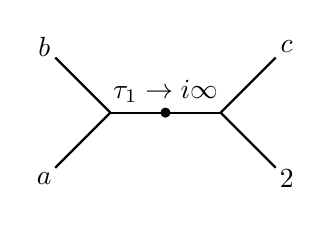
\begin{tikzpicture}[thick,scale=0.7]
  \node at (-.2,.2) {$b$};
  \node at (-.2,-2.2) {$a$};
  \node at (4.2,.2) {$c$};
  \node at (4.2,-2.2) {$2$};
  \draw[-](0,0)--(1,-1);
  \draw[-](1,-1)--(0,-2);
  \draw[-](1,-1)--(2,-1);
  \draw[-](2,-1)--(3,-1);
  \draw[-](3,-1)--(4,0);
  \draw[-](3,-1)--(4,-2);
  \filldraw[black] (2,-1) circle (2pt) node[above]{$\tau_{1}\rightarrow i \infty$};
\end{tikzpicture}\qquad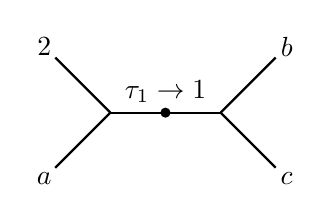
\begin{tikzpicture}[thick,scale=0.7]
  \node at (-.2,.2) {$2$};
  \node at (-.2,-2.2) {$a$};
  \node at (4.2,.2) {$b$};
  \node at (4.2,-2.2) {$c$};
  \draw[-](0,0)--(1,-1);
  \draw[-](1,-1)--(0,-2);
  \draw[-](1,-1)--(2,-1);
  \draw[-](2,-1)--(3,-1);
  \draw[-](3,-1)--(4,0);
  \draw[-](3,-1)--(4,-2);
  \filldraw[black] (2,-1) circle (2pt) node[above]{$\tau_{1}\rightarrow 1$};
\end{tikzpicture}\qquad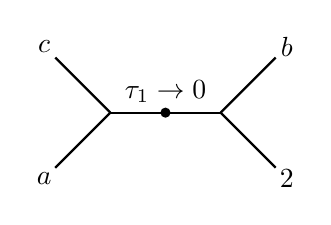
\begin{tikzpicture}[thick,scale=0.7]
  \node at (-.2,.2) {$c$};
  \node at (-.2,-2.2) {$a$};
  \node at (4.2,.2) {$b$};
  \node at (4.2,-2.2) {$2$};
  \draw[-](0,0)--(1,-1);
  \draw[-](1,-1)--(0,-2);
  \draw[-](1,-1)--(2,-1);
  \draw[-](2,-1)--(3,-1);
  \draw[-](3,-1)--(4,0);
  \draw[-](3,-1)--(4,-2);
  \filldraw[black] (2,-1) circle (2pt) node[above]{$\tau_{1}\rightarrow 0$};
\end{tikzpicture}
\end{equation}
which are exchanged by triality operation. So on the full theory, the triality acts as follows (where we can do the same job on the other coupling).

If the moduli space is really the product of two UHP we should be able to do S-duality on both nodes one after the other and viceversa and get the same result. 
\begin{figure}[H]
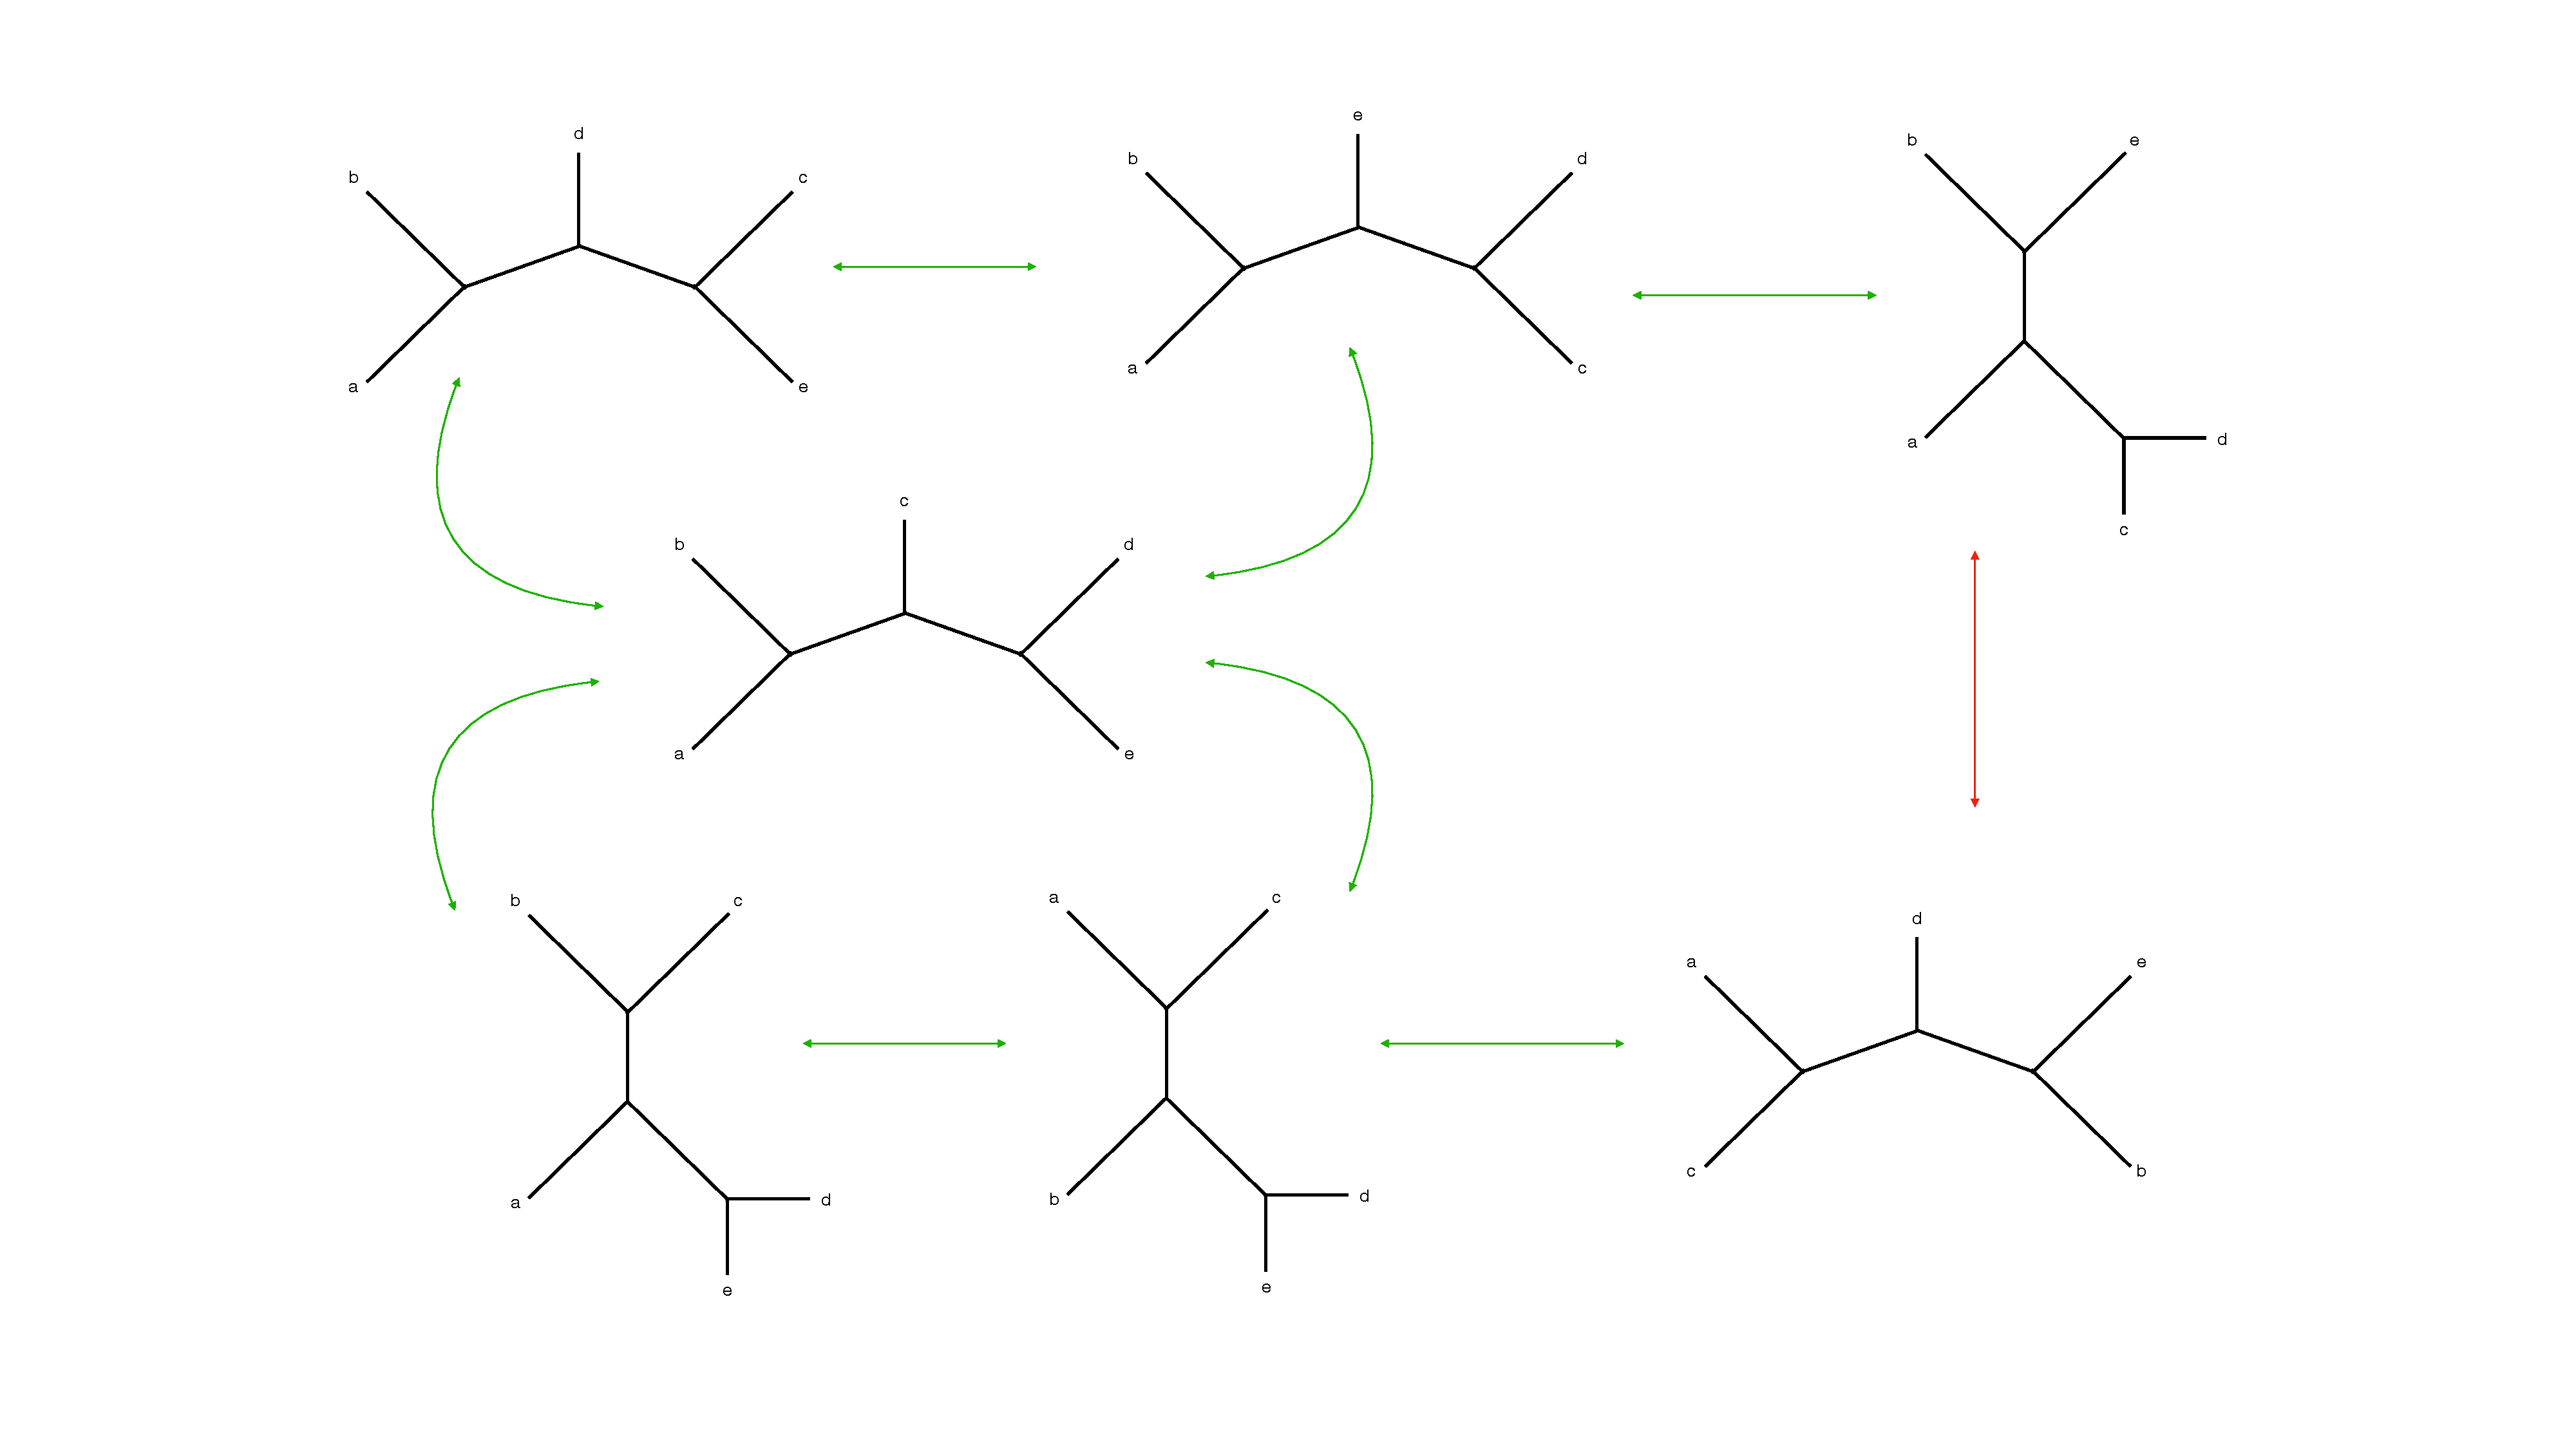
\includegraphics[width=\textwidth]{dualities.pdf}
\end{figure}
But what happens is that the two are not the same. But the two are related by S-duality. We found a pentagon of dualities. Here one gets a polytope made up of pentagons and triangles: the boundary of the parameter space (permutahedron, all the ways one can permute the $5$ flavour symmetries $5!/4$). So the hypotesis of the two UHP is wrong.

So what happens to a generic theory $T_{\Gamma}$? We have some trivalent graph and each S-duality operation reorganizes the four legs that come out of a segment. Through this basic operations we can relate all graphs with the same number of external leaves and loops (number of loops $g$ gives formula for dimension of Coulomb branch of the theory). There is a big moduli space $M_{g,n}$ (generalize notion of modular region?) of some $4d$ SCFT which with many cusps on the bundary each looking with some lagrangian description of $T_{\Gamma}$ with $g$ loops and $n$ leaves.\\
This $M_{g,n}$ has a bunch of charts in which I have a trivalent graph $\Gamma$ and a bunch of coordinates for each edge. Each chart looks like the upper region of the product of two UHP. But we want to combine all this charts together to glue the charts using S-dualities. This reminds us of Riemann surfaces. Instead of trying to build this $M_{g,n}$ by hand, I can see that there is a very famous moduli space with exactly the right dimension and properties. This is the space of complex structures of Riemann surfaces of genus $g$ with $n$ punctures. Let us see if we can really write charts which are naturally parametrized by the gauge couplings of my lagrangian.

Suppose to have a certain trivalent graph $\Gamma$. Associate to this graph a bunch of spheres with three marked points. We want to build out a Riemann surface of genus $g$ and $n$ punctures. There is a pretty natural way of doing it: every time I want to glue together two spheres to have a sensible Riemann surface which makes out my graph. What I can do is take some local coordinate system around this marked point and some local coordinates $z_{1}$ which goes to zero at the point. Take another one on the other sphere $z_{2}$ which goes together on the other marked point. To glue them together we declare that the following is satisfied
\begin{equation}
	z_{1}z_{2}=q
\end{equation}
where $q$ is some parameter. When $q=0$ we get the equation for two separate planes (so the two surfaces are disjoint and only touch at one point), with different $q$ they start merging together. So there is a certain patch in parameter space in the Riemann surface which has this coordinate system given by the $q_{i}$. To make sure is a good coordinate patch we should have $3g-3+n$ $q_{i}$s, and this number is the dimension of the moduli space of complex structures of the Riemann surface. As $q_{i}\rightarrow 0$ we get spheres which are connected together by very thin tubes.

We now claim that 
\begin{equation}
	q_{i}=e^{2\pi i\tau_{i}}
\end{equation}
so that the basic shift of the $\theta$ angle leaves the $q_{i}$ invariant. Now we need to see if it makes sense, especially for the S-duality transformation.

Take $\SU(2)$ with $N_{f}=4$. I can glue two spheres in two ways to get two patches in the moduli space of the theory
\begin{figure}[H]
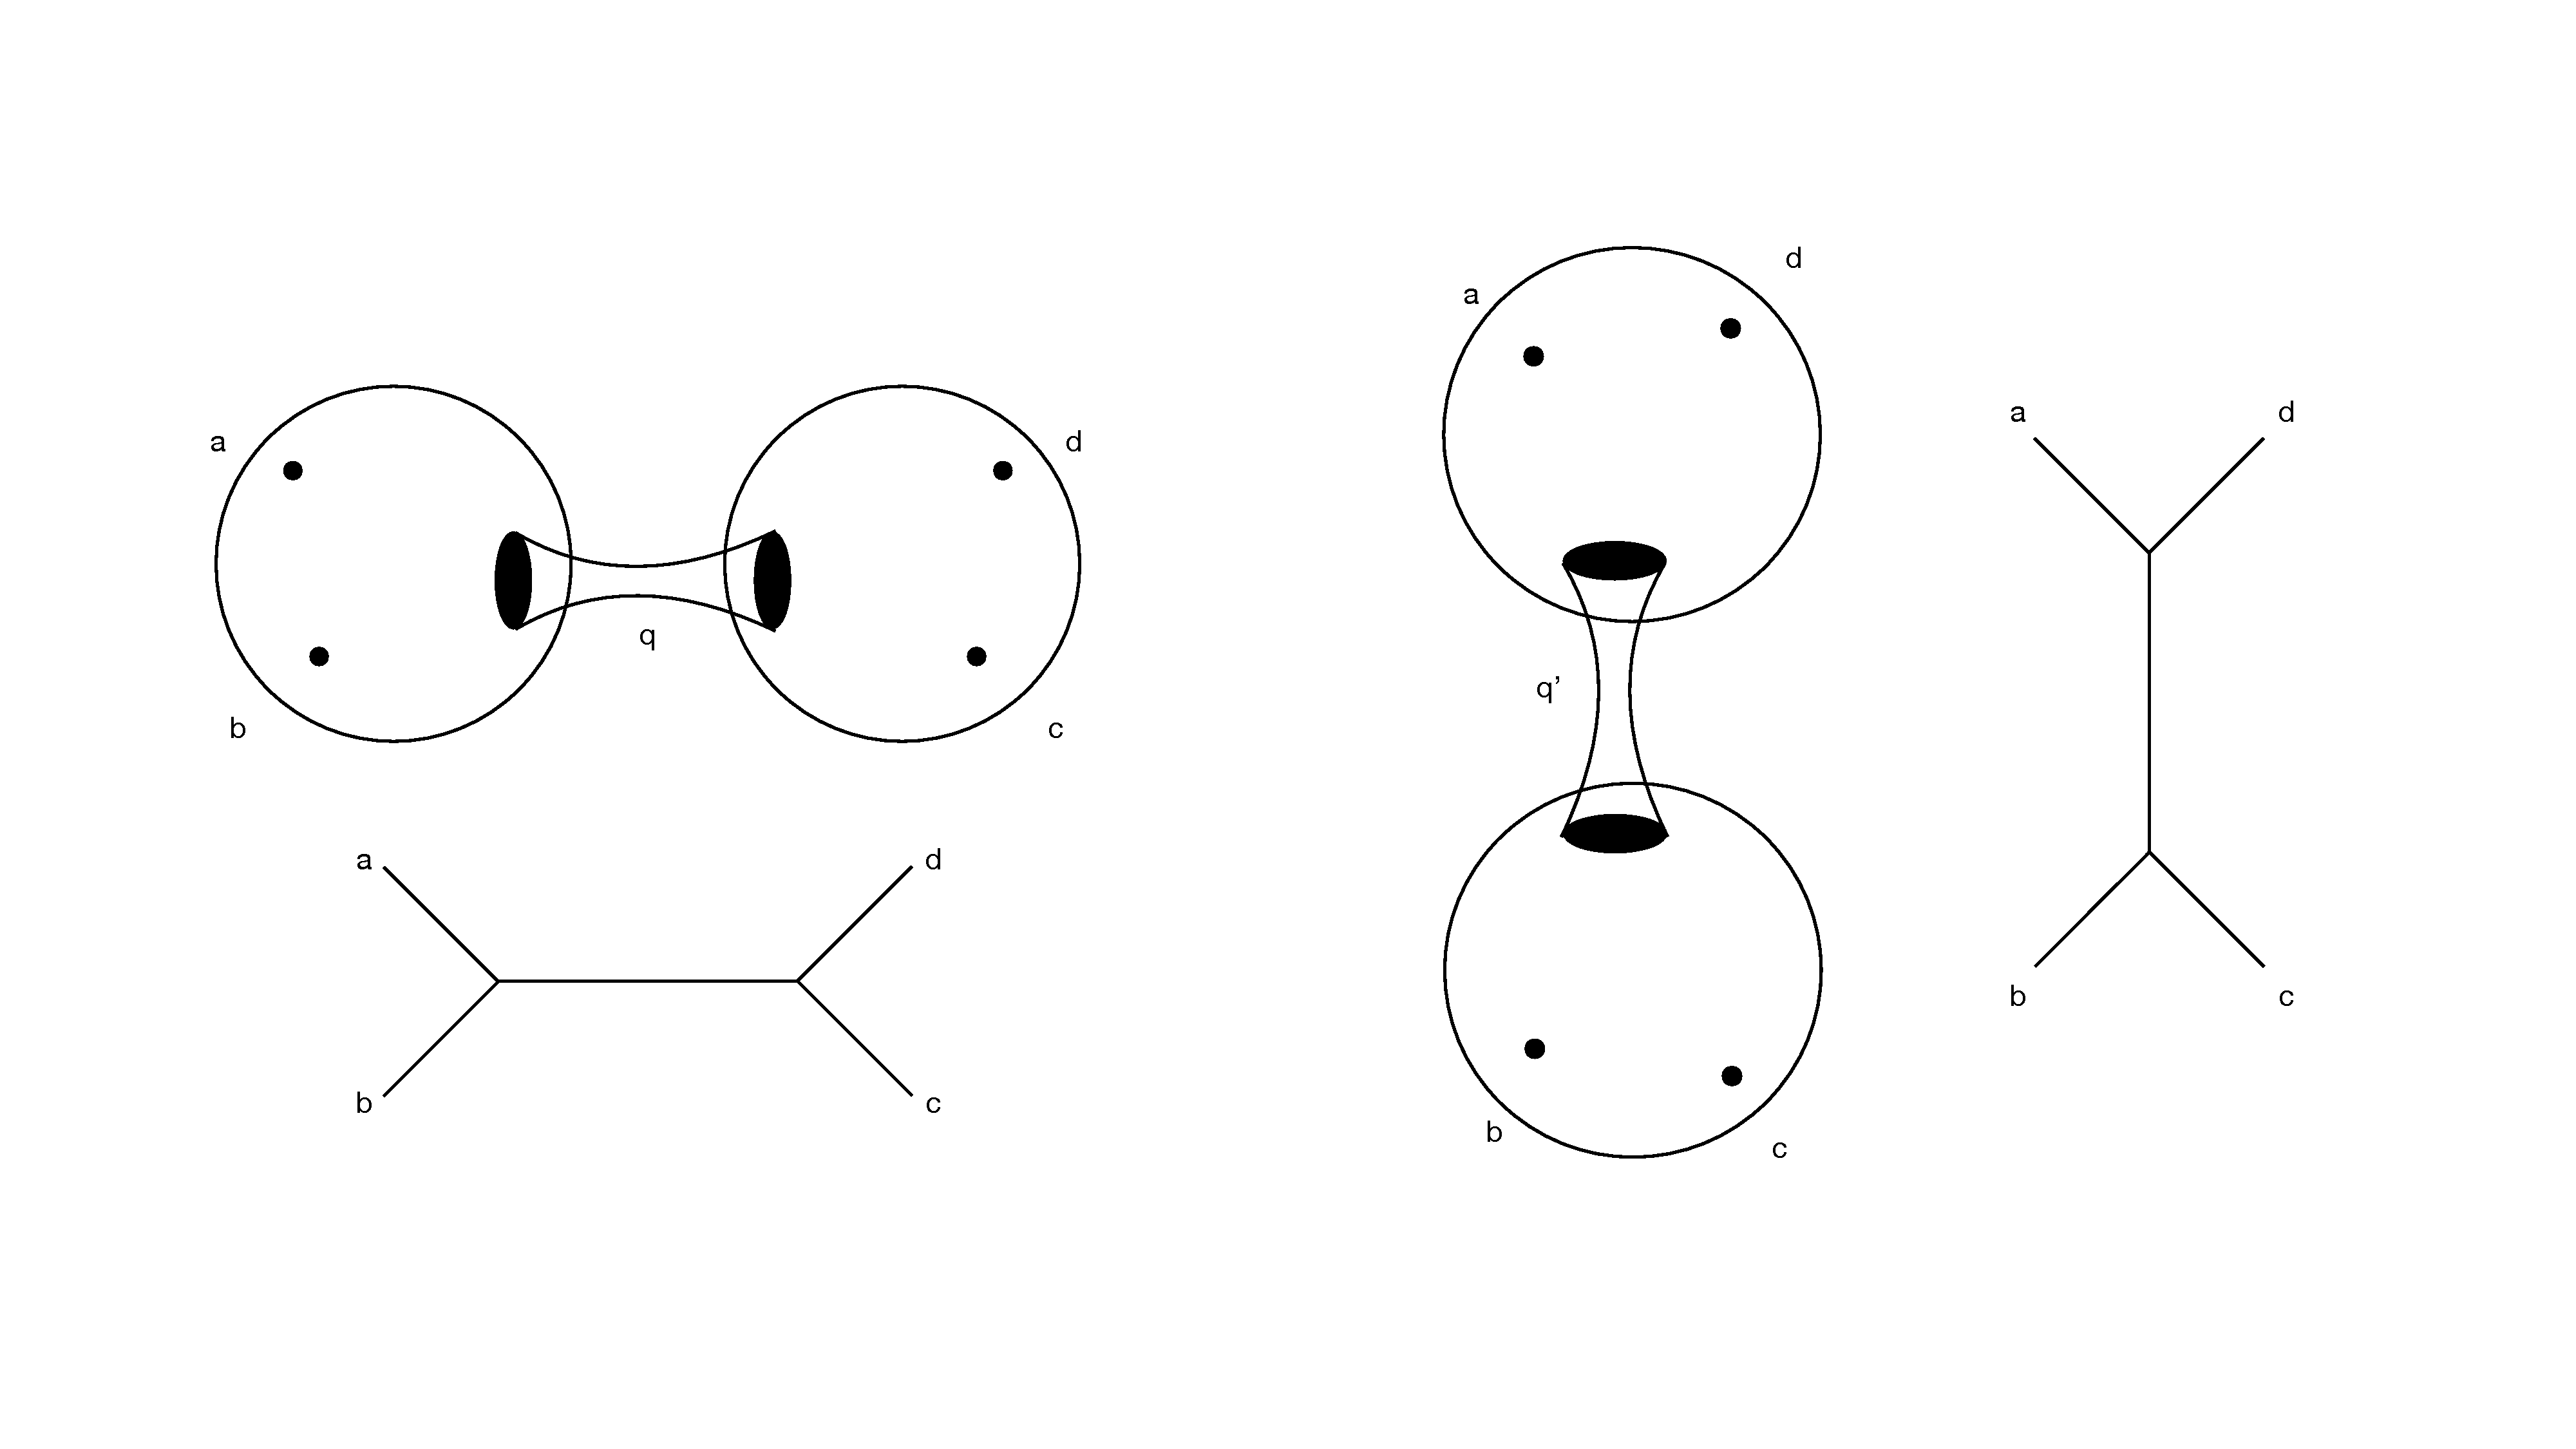
\includegraphics[width=\textwidth]{su2.pdf}
\end{figure}
The Riemann surface that we make with this gluing is just a sphere with four punctures. Suppose to put the puctures at $0,1,\infty$ where we picked some global coordinates on the spheres $z,w$ (Riemann sphere is $\bbC$). The gluing is just 
\begin{equation}
	\frac{z}{w}=q
\end{equation}
In the $w$ plane we have points at $0,1,q,\infty$. We wanted our parameter space to look like a UHP a (moduli space of the torus). Is very easy to make a torus out of a four punctured sphere: write the equation $y^{2}=P(z)$ where $P(z)$ is some polynomial with zeros at that four points
\begin{equation}
	y^{2}=z(z-1)(z-q)
\end{equation}
This describes an elliptic curve, a torus. The torus has a certain modular parameter $\tau(q)$. When comparing the three possibilities for the three theories one finds
\begin{equation}
	q\rightarrow1-q^{\prime},\qquad q\rightarrow\frac{1}{q^{\prime\prime}}
\end{equation}
and converting them to statements in $\tau$ they become exactly $\SL(2,\bbZ)$ transformations. The three patches really coincide with the three possible theories.

With this picture we can describe easily the moduli space. For example the (\ref{eq:N4}) graph, beign $\cN=4$ SYM is identified by taking the three-punctured sphere and connecting together two punctures $1,\infty$. In the $\bbC$ plane this looks like taking an annulus and connecting together the boundaries to make a torus. The modular parameter of the torus is then exactly the marginal coupling of $\cN=4$ SYM.

Now one would like to know that, now that we know the boundaries of the moduli space, there is going to be no problem going in. Since complex geometry is very strict we would expect it to work. To do so one should build the Seiberg-Witten curves and check that they really behave properly on the parameters (the IR lagrangian at each point).

So take above each point the Coulomb branch of the theory and check that it is fiberd properly and that it transforms well under S-dualities. Moreover the dimension of the CB is $3g-3+n$ which happens to be exactly as the dimension of the parameter space. This is not a coincidence: if you want to change the gauge coupling, you just need to change the lagrangian by adding a prepotential term
\begin{equation}
	L+\delta\tau_{i}\int \Tr\phi_{i}^{2}
\end{equation}
the expectation value of which is a coordinate on the CB $u_{i}$. Viceversa, every dimension two operator could be added to the lagrangian to give a coupling. So coupling and dimension two operators are in one-to-one correspondence. More is pretty clear that $u_{i}\delta\tau_{i}$ should be a 1-form, so should transform as a 1-form and this tells us how the CBs in each patches should be glued together. It should be glued together the same way as the cotangent bundle of $M_{g}$, $T^{*}M_{g}$. So the CB should be fiberd the same way as the cotangent bundle.

There is a very cute way to describe the cotangent bundle to a Riemann surface. First of all we should get a good way to describe $\tau_{i}$. How do I change the $q$s? I cut and then glue together again: take a path $\gamma$ and cut along the path and I glue it back after acting with a vector field which acts in a neighborhood of $\gamma$. Local transformation
\begin{equation}
	\delta\tau_{i}v^{i}\pdv{}{z}
\end{equation}
Quadratic differentials with single poles are just deformations in the coulomb branch. If one includes mass parameters on the punctures, the differential should have a double pole on the puncture.